\documentclass[12pt,twoside,spanish,a4paper]{report}

\usepackage[T1]{fontenc}
\usepackage[spanish]{babel}
\usepackage[latin1]{inputenc}

%\usepackage{geometry}
%\geometry{verbose,a4paper,tmargin=2.0cm,bmargin=2.0cm,lmargin=2.0cm,rmargin=2.0cm}

\usepackage{a4wide}

\usepackage{graphicx}
\usepackage{longtable}
\usepackage{array,ae,aeguill,picins}
\usepackage{amsmath,amsfonts,amssymb}
\usepackage{pstricks,pst-all}
\usepackage{color}

\title{Diez lecciones para descubrir el lenguaje \textsc{Logo}}
\author{Lo\"ic Le Coq. Traducci\'on: \'Alvaro Vald\'es} % y Marcelo Dushkin}
\date{\texttt{http://xlogo.tuxfamily.org}}

\begin{document}

\maketitle

\newpage

\tableofcontents{}

\newpage{}

\chapter*{Introducci\'on}

En este manual encontrar\'a una serie de \textit{recetas} que le ayudar\'an a
aprender el lenguaje \textsc{Logo}. \\

Soy profesor de matem\'aticas, y esta gu\'ia es una peque\~na compilaci\'on
de las distintas actividades realizadas en clase con los alumnos de
clase de cuarto y quinto. Cada secci\'on intenta abordar un concepto
particular del lenguaje y propone actividades que deben realizarse,
o bien como descubrimiento o como autoevaluaci\'on (en este caso,
est\'an disponibles algunas soluciones al final del tutorial). \\

Este manual no pretende ser EL tutorial ideal para comprender \textsc{Logo}.
Se limita a proponer distintas pistas, distintos enfoques sobre algunos
aspectos de la programaci\'on en \textsc{Logo}. Las actividades son
de niveles variados y, creo, representan un buen conjunto de experiencias
de lo que es capaz de realizar el lenguaje \textsc{Logo}. !`Espero
que las explicaciones aportadas sean lo m\'as claras posibles! No duden
en hacerme llegar sus comentarios y sus cr\'iticas respecto a este tutorial.
Y ahora, !`a iniciarse a las alegr\'ias de la peque\~na tortuga!

\newpage{}

\chapter{Descubramos las primitivas b\'asicas}
   \label{sec:Descubrir-las-primitivas}

Para desplazar a la tortuga sobre la pantalla, se utilizan \'ordenes
predefinidas llamadas \char`\"{}primitivas\char`\"{}. En esta primera
secci\'on, se van a describir las primitivas b\'asicas que permiten controlar
a la tortuga.

\section{Primeras primitivas que utilizaremos}
   \label{sub:Nuevas-primitivas}

\begin{itemize}
   \item \texttt{avanza n\'umero\hspace{3.8cm} \textcolor{red}{av 50}}

      Hace avanzar a la tortuga el n\'umero de pasos indicado
   \item \texttt{retrocede n\'umero\hspace{3.3cm} \textcolor{red}{re 100}}

      Hace retroceder a la tortuga el n\'umero de pasos indicado
   \item \texttt{giraderecha n\'umero\hspace{2.9cm} \textcolor{red}{gd 90}}

      La tortuga gira a la derecha el \'angulo indicado
   \item \texttt{giraizquierda n\'umero\hspace{2.7cm} \textcolor{red}{gi 90}}

      La tortuga gira a la izquierda el \'angulo indicado
   \item \texttt{borrapantalla \hspace{4cm} \textcolor{red}{bp}}

      Borra la pantalla y devuelve a la tortuga al centro de la pantalla
      (vuelve al origen)
   \item \texttt{muestratotuga \hspace{4.1cm} \textcolor{red}{mt}}

      Hace visible a la tortuga en la pantalla
   \item \texttt{ocultatortuga \hspace{4.1cm} \textcolor{red}{ot}}

      Oculta la tortuga. Permite una visualizaci\'on mas r\'apida.
   \item \texttt{subelapiz \hspace{5.0cm} \textcolor{red}{sl}}

      Sube el \char`\"{}l\'apiz\char`\"{}. La tortuga no deja trazo tras
      ella (no dibuja) cuando se desplaza.
   \item \texttt{bajalapiz \hspace{5.0cm} \textcolor{red}{bl}}

      Baja el l\'apiz. La tortuga escribe cuando se desplaza.
   \item \texttt{repite n\'umero lista \hspace{2.7cm}
      \textcolor{red}{repite 5 [av 50 gd 45]}}

      Repite las instrucciones contenidas en la lista el n\'umero de veces
      indicado
\end{itemize}

\section{Dibujar un pol\'igono regular}
   \label{sub:Dibujar-poligono}

\noindent Vamos a aprender a dibujar un cuadrado, un tri\'angulo equil\'atero,
un pent\'agono regular, etc.

\subsection{El cuadrado}
   \label{sub:El-cuadrado}

En el dibujo siguiente, un cuadrado representa 50 \char`\"{}pasos\char`\"{}
de tortuga.
\begin{center}
   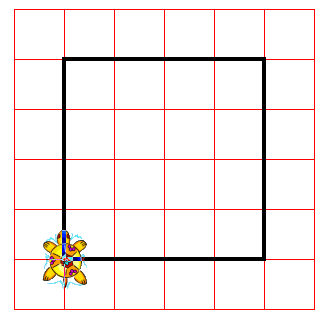
\includegraphics[scale=0.4]{Imagenes_Tutorial/01_Cuadrado.png}
\end{center}

\noindent Para dibujar el cuadrado de la figura, se debe escribir:
\begin{verbatim}
  avanza 200 giraderecha 90
  avanza 200 giraderecha 90
  avanza 200 giraderecha 90
  avanza 200 giraderecha 90 \end{verbatim}
Date cuenta que se repite 4 veces la misma instrucci\'on, as\'i que podemos
usar una sintaxis m\'as r\'apida:
\begin{verbatim}
 repite 4 
   [ av 200 gd 90 ] \end{verbatim}

\subsection{El tri\'angulo equil\'atero}
   \label{sub:El-triangulo}

% \input{Imagenes_pstricks/02_triangulo}
Vamos a ver c\'omo trazar este tri\'angulo equil\'atero de 180 pasos de
tortuga:
\begin{center}
   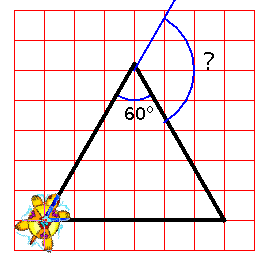
\includegraphics[scale=0.5]{Imagenes_Tutorial/02_Triangulo.png}

   Aqu\'i, un cuadrado representa 30 pasos de tortuga
\end{center}

\noindent Las \'ordenes ser\'an algo del estilo:
\begin{verbatim}
  repite 3
    [ avanza 180 giraderecha ... ] \end{verbatim}
Queda por determinar el \'angulo correcto. En un tri\'angulo equil\'atero,
los \'angulos valen todos 60 grados, y como la tortuga debe volver por el
exterior del tri\'angulo, el \'angulo valdr\'a:
\begin{center}
  \texttt{180 - 60 = 120 grados}
\end{center}
Las \'ordenes son, pues:
\begin{verbatim}
  repite 3
    [ av 180 gd 120 ] \end{verbatim}

\subsection{El hex\'agono}
    \label{sub:El-hexagono}

% \input{Imagenes_pstricks/03_hexagono}
\begin{center}
   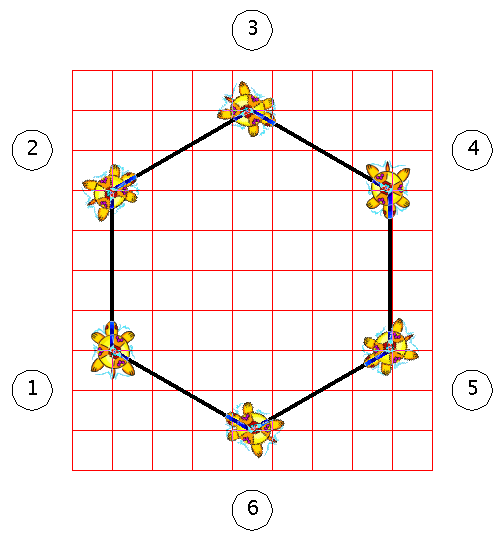
\includegraphics[scale=0.3]{Imagenes_Tutorial/03_Hexagono}

   Un cuadrado = 20 pasos de tortuga.
\end{center}

Para un cuadrado repet\'iamos 4 veces, para el tri\'angulo 3 veces, parece
claro que para el hex\'agono ser\'a:
\begin{verbatim}
  repite 6
    [ avanza 80 giraderecha ... ] 
\end{verbatim}
Date cuenta que en su desplazamiento, la tortuga realmente da una
vuelta completa sobre ella misma. (Inicialmente est\'a orientada hacia
arriba y termina en esta misma posici\'on). Esta rotaci\'on de 360 grados
se efect\'ua en 6 etapas. Por tanto, cada vez, gira
\begin{center}
   \texttt{360/6 = 60 grados}
\end{center}
Las \'ordenes son, entonces:
\begin{verbatim}
  repite 6
    [ av 80 gd 60 ] \end{verbatim}
%?`Va quedando claro el proceso?

\subsection{Trazar un pol\'igono regular en general}
   \label{sub:Trazar-poligono}

En realidad, reiterando el razonamiento anterior, puedes darte cuenta
de que para trazar un pol\'igono de \texttt{n} lados, el \'angulo se obtendr\'a
dividiendo \texttt{360} por \texttt{n}. Por ejemplo:
\begin{itemize}
   \item Para trazar un pent\'agono regular de lado \texttt{100}:
      \texttt{(360:5=72)} 
      \begin{verbatim}
 repite 5 [ av 100 gd 72 ] \end{verbatim}
   \item Para trazar un ene\'agono regular de lado \texttt{20}:
      \texttt{(360:9=40)}
      \begin{verbatim}
 repite 9 [ av 20 gd 40 ] \end{verbatim}
   \item Para trazar un eh \ldots{} \texttt{360-}gono%
      \footnote{Trihectahexacont\'agono:
                tri = 3, hecta = 100, hexaconta = 60,
                gono = \'angulo}
      regular de lado \texttt{2} (que se parece mucho a un c\'irculo):
      \begin{verbatim}
 repite 360 [ av 2 gd 1 ] \end{verbatim}
   \item Para trazar un hept\'agono regular de lado \texttt{120}:
      \begin{verbatim}
 repite 7 [ av 120 gd 360/7 ] \end{verbatim}
\end{itemize}

\section{Empezando con procedimientos}
   \label{sub:Procedimientos}

Para evitar tener que repetir cada vez las instrucciones para dibujar
un cuadrado, un tri\'angulo \ldots{}, puedes definir instrucciones
personalizadas llamadas \char`\"{}procedimientos\char`\"{}. Un procedimiento
comienza con la palabra clave \texttt{para} y termina con la palabra
clave \texttt{fin}. Por ejemplo, abre el editor, escribe:
\begin{verbatim}
  para cuadrado
    repite 4
      [ avanza 100 giraderecha 90 ]
  fin \end{verbatim}
\noindent luego cierra al editor guardando los cambios haciendo
\textit{click} en el ping\"uino. Ahora cada vez que se escriba
\texttt{cuadrado}, !`un cuadrado aparecer\'a en la pantalla!

\section{Actividad}
   \label{sub:Actividad_Casa}

% \input{Imagenes_pstricks/04_casa}
Debes conseguir el dibujo que se muestra a continuaci\'on.
\begin{center}
   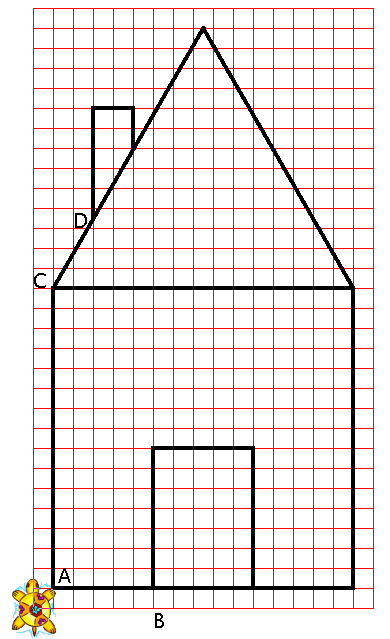
\includegraphics[scale=0.5]{Imagenes_Tutorial/04_Casa.png}

   Cada cuadrado vale 10 pasos de tortuga.
\end{center}
Para ello, deber\'as definir ocho procedimientos:
\begin{itemize}
   \item Un procedimiento \char`\"{}\texttt{cuadrado}\char`\"{} que trazar\'a
      el cuadrado b\'asico de la casa
   \item Un procedimiento \char`\"{}\texttt{tri}\char`\"{} que trazar\'a el
      tri\'angulo equil\'atero que representa el tejado %de la casa
   \item Un procedimiento \char`\"{}\texttt{puerta}\char`\"{} que trazar\'a el
      rect\'angulo que representa la puerta %de la casa
   \item Un procedimiento \char`\"{}\texttt{chi}\char`\"{} que trazar\'a la
      chimenea
   \item Un procedimiento \char`\"{}\texttt{desp1}\char`\"{} que desplazar\'a la
      tortuga de la posici\'on A a la B
   \item Un procedimiento \char`\"{}\texttt{desp2}\char`\"{} que llevar\'a a la
      tortuga desde la posici\'on B a la C
   \item Un procedimiento \char`\"{}\texttt{desp3}\char`\"{} que har\'a a la
      tortuga ir de la posici\'on C a la D
   \item Un procedimiento \char`\"{}\texttt{casa}\char`\"{} que trazar\'a la
      casa en su totalidad ayud\'andose de todos los dem\'as procedimientos
\end{itemize}

\newpage{}

\chapter{Utilizando las coordenadas}
    \label{sec:Utilizando-coordenadas}

\section{Presentaci\'on}
   \label{sub:Presentacion}

% \input{Imagenes_pstricks/05_coordenadas}
En esta secci\'on, vamos a descubrir la primitiva \texttt{ponposicion}.

%\parbox{10cm}{
El \textbf{\'Area de Dibujo} es un sistema cartesiano cuyo origen est\'a
situado en el centro de la pantalla. De este modo, podemos alcanzar
cualquiera de los puntos de dicho \'area ayudados por sus coordenadas.\\

\noindent La primitiva que vamos a utilizar es:

\texttt{ponposicion lista \hspace{2cm} \textcolor{red}{ponpos [100 -250]}}

\noindent que desplaza la tortuga al punto cuyas coordenadas son las definidas
en la lista. \\

\noindent Un ejemplo sencillo de su utilizaci\'on:
\begin{verbatim}
   borrapantalla
   ponpos [200 100]
   ponpos [50 -150]
   ponpos [-100 -150] \end{verbatim}
\begin{center}
   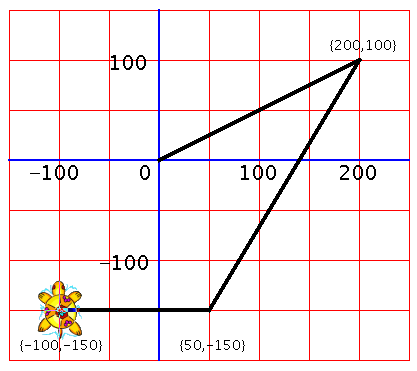
\includegraphics[scale=0.5]{Imagenes_Tutorial/05_Coordenadas.png}
\end{center} %}

\section{Actividad}
   \label{sub:Actividad-Policubos}

% \input{Imagenes_pstricks/06_policubos}
En esta actividad debes realizar la siguiente figura.
\begin{center}
   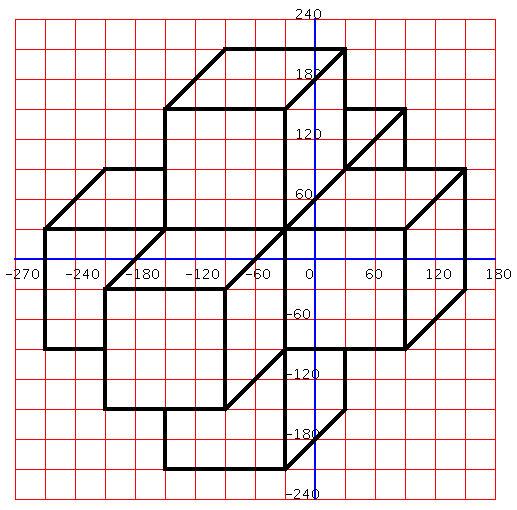
\includegraphics[scale=0.5]{Imagenes_Tutorial/06_Policubo.png}
\end{center}
S\'olo puedes utilizar las primitivas
\begin{itemize}
   \item \texttt{ponposicion} (\texttt{ponpos})
   \item \texttt{borrapantalla} (\texttt{bp})
   \item \texttt{subelapiz} (\texttt{sl})
   \item \texttt{bajalapiz} (\texttt{bl})
\end{itemize}

\newpage{}

\chapter{Las variables}
   \label{sec:Las-variables}

\section{Papel de las variables}
   \label{sub:Papel-variables}

A veces, se desear\'ia dibujar una misma forma pero con dimensiones
diferentes. Por ejemplo, si se desea dibujar un cuadrado de lado 100,
un cuadrado de lado 200 y un cuadrado de lado 50, con lo que sabemos
hasta ahora deber\'iamos definir tres procedimientos diferentes, uno
para cada uno de estos cuadrados. Ser\'ia m\'as simple definir un \'unico
procedimiento al que se pasara como par\'ametro la longitud deseada
del lado. Por ejemplo, \texttt{cuadrado 200} trazar\'ia el cuadrado
de lado 200, \texttt{cuadrado 100} trazar\'ia el cuadrado de lado 100,
etc. Eso es precisamente lo que las variables nos van a permitir realizar.

\section{Ejemplos de utilizaci\'on}
    \label{sub:Ejemplos-uso-variables}

% \input{Imagenes_pstricks/07_cuadrados}
\noindent Para dibujar un cuadrado de lado \texttt{100}, hab\'iamos escrito:
\begin{verbatim}
  para cuadrado
    repite 4
      [ avanza 100 giraderecha 90]
  fin \end{verbatim}
Vamos a modificar este procedimiento para que reciba un par\'ametro
(o dicho de forma elegante, un \char`\"{}argumento\char`\"{}) que
indique la longitud del lado del cuadrado a dibujar. \\
Una variable siempre va precedida del s\'imbolo \char`\"{}\texttt{:}\char`\"{}.
Si queremos indicar al procedimiento \texttt{cuadrado} que dependa
de la variable \texttt{:c}, se a\~nade a la l\'inea de definici\'on la ruta
\texttt{:c}. \\

En consecuencia, no debemos indicar a la tortuga que avance \texttt{100} pasos,
sino \texttt{:c} pasos. El procedimiento resultante es:
\begin{verbatim}
  para cuadrado :c
    repite 4
      [ avanza :c giraderecha 90]
  fin \end{verbatim}
\noindent As\'i, escribiendo:
\begin{verbatim}
   bp ot cuadrado 100 cuadrado 50 cuadrado 30 cuadrado 20 cuadrado 10  \end{verbatim}
Obtenemos la figura siguiente:
\begin{center}
   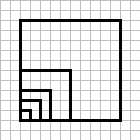
\includegraphics[scale=0.5]{Imagenes_Tutorial/07_Cuadrados.png}
\end{center}

\section{Trazar un rect\'angulo de altura y anchura determinadas}
   \label{sub:Trazar-un-rectangulo}

Definamos ahora un procedimiento llamado \texttt{rectangulo} que depender\'a
de dos variables. Por ejemplo, \texttt{rec 200 100} trazar\'a un rect\'angulo
de altura \texttt{200} y anchura \texttt{100}. Para ello:
\begin{verbatim}
   para rectangulo :alto :ancho
     repite 2
       [ avanza :alto giraderecha 90 avanza :ancho giraderecha 90 ]
   fin \end{verbatim}
Hechos los cambios:
\begin{verbatim}
   borrapantalla ocultatortuga
   rectangulo 200 100 rectangulo 100 300
   rectangulo  50 150 rectangulo  10  20
   rectangulo 140  30 \end{verbatim}
genera:
\begin{center}
   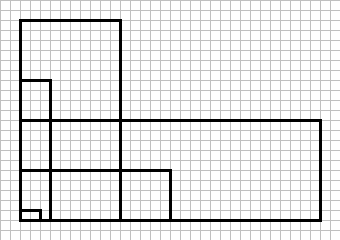
\includegraphics[scale=0.5]{Imagenes_Tutorial/07_rectangulos.png}
\end{center}

Ahora bien, si no se proporciona alguno de los argumentos al procedimiento
\texttt{rectangulo}, el int\'erprete nos indicar\'a con un mensaje de error que
el procedimiento necesita otro argumento:

\textcolor{red}{\texttt{No hay suficientes datos para  rectangulo}}

\section{Trazar una forma con distintos tama\~nos}
   \label{sub:Trazar-forma}

Veamos como trazar un cuadrado y un rect\'angulo con dos tama\~nos distintos.
Ahora volvamos al ejemplo de la casa de la secci\'on \ref{sub:Actividad_Casa}
y c\'omo modificar el c\'odigo para dibujar la casa sin que importen las
dimensiones.

El objetivo es pasar un argumento al procedimiento \texttt{casa} para
que, seg\'un el par\'ametro, la casa sea m\'as o menos grande. Has de notar
que:
\begin{itemize}
   \item \texttt{casa 10} dibujar\'a la casa de la secci\'on
      \ref{sub:Actividad_Casa}.
   \item \texttt{casa 5} dibujar\'a la casa a escala 0,5.
   \item \texttt{casa 20} dibujar\'a una casa con las dimensiones dos
      veces m\'as grandes
\end{itemize}
La noci\'on de proporcionalidad se da por conocida. Seg\'un el dibujo
de la secci\'on \ref{sub:Actividad_Casa}, un cuadrado representa 10
pasos. El procedimiento \texttt{cuadrado} era el siguiente:
\begin{verbatim}
  para cuadrado
    repite 4
      [ avanza 150 giraderecha 90 ]
  fin \end{verbatim}
\noindent que ahora se va a convertir en:
\begin{verbatim}
  para cuadrado :c
    repite 4
      [ avanza :c giraderecha 90 ]
  fin \end{verbatim}
As\'i, cuando se escriba \texttt{cuadrado 10}, el cuadrado tend\'a un
lado igual a \texttt{15 * 10 = 150}. !`Las proporciones se mantienen
correctamente!  De hecho, hay que darse cuenta de que va a ser necesario
reescribir todos los procedimientos y cambiar las longitudes de desplazamiento
de la siguiente manera.
\begin{itemize}
   \item \texttt{70} se convertir\'a en \texttt{7 * :c}
   \item \texttt{av 45} se convertir\'a en \texttt{av 4.5 * :c}
   \item etc.
\end{itemize}
Eso hace que, en realidad, !`s\'olamente haya que contar el n\'umero de
cuadrados para cada longitud! Se obtiene:
\begin{verbatim}
  para cuadrado :c
    repite 4
      [ avanza 15*:c giraderecha 90 ]
  fin

  para tri :c
    repite 3
      [ avanza 15*:c giraderecha 120 ]
  fin

  para puerta :c
    repite 2
      [ avanza 7*:c giraderecha 90
        avanza 5*:c giraderecha 90 ]
  fin

  para chi :c
    avanza 5.5*:c giraderecha 90
    avanza 2*:c giraderecha 90
    avanza 2*:c
  fin

  para desp1 :c
    subelapiz
    giraderecha 90 avanza 5*:c
    giraizquierda 90
    bajalapiz
  fin

  para desp2 :c
    subelapiz
    giraizquierda 90 avanza 5*:c
    giraderecha 90 avanza 15*:c
    giraderecha 30
    bajalapiz
  fin

  para desp3 :c
    subelapiz
    giraderecha 60 avanza 2*:c
    giraizquierda 90 avanza 3.5*:c
    bajalapiz
  fin

  para casa :c
    cuadrado :c desp1 :c puerta :c desp2 :c tri :c desp3 :c chi :c
  fin \end{verbatim}

\section{Actividad}
   \label{sub:Actividad-Robot-Rana}

Realiza los siguientes dibujos con dos variables de modo que sea posible
obtenerlos a distintos tama\~nos: \\

% \input{Imagenes_pstricks/08_robot}
\noindent \begin{center}
   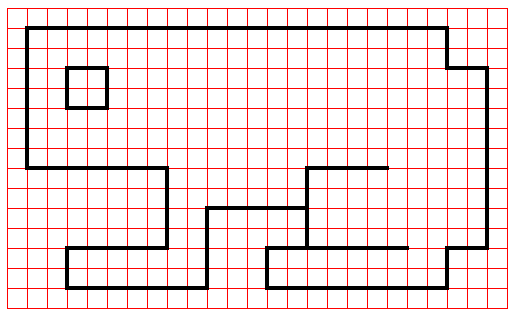
\includegraphics[scale=0.5]{Imagenes_Tutorial/09_Ranita.png}
\end{center}
\vspace{2cm}
% \input{Imagenes_pstricks/09_ranita}
\noindent \begin{center}
   \includegraphics%[width=15.0cm,keepaspectratio]
      {Imagenes_Tutorial/08_Robot.png}
\end{center}

%\noindent \begin{center}
%   \includegraphics[scale=0.4]{Imagenes_Tutorial/08_robot}
%
%   \includegraphics[scale=0.4]{Imagenes_Tutorial/09_ranita}
%\end{center}

\newpage{}

\chapter{La recursividad}
    \label{sec:La-recursividad}

Se dice que un procedimiento es recursivo si se llama a s\'i mismo.
Veamos algunos ejemplos que utilizan esta propiedad.

\section{En el \'Area de Dibujo}
   \label{sub:Recursividad-Area-Dibujo}

\subsection{Primer ejemplo}
   \label{sub:Primer-ejemplo}

Escribe el siguiente procedimiento en el Editor:
\begin{verbatim}
  para ejemplo1
    giraderecha 1
    ejemplo1
  fin \end{verbatim}
Este procedimiento es recurrente puesto que se ejecuta la orden
\texttt{ejemplo1} en la \'ultima linea. En la ejecuci\'on, se comprueba que
la tortuga no deja de girar sobre s\'i misma. Para parar el programa, nos
vemos obligados a hacer click en el boton \texttt{Alto}.

\subsection{Tres nuevas primitivas}
   \label{sub:Tres-nuevas-primitivas}

\begin{itemize}
   \item \texttt{espera n\'umero \hspace{3cm} \textcolor{red}{espera 60}}

      Hace una pausa igual a la 60"a parte del n\'umero indicado.

      Por ejemplo, \texttt{espera 120} deja el programa parado durante dos
      segundos
   \item \texttt{goma \hspace{5cm} \textcolor{red}{go}}

      Cuando la tortuga se desplaza, borra todo a su paso en vez de dejar
      un rastro tras ella
   \item \texttt{ponlapiz \hspace{4.2cm} \textcolor{red}{pla}}

      Devuelve al modo de dibujo habitual: la tortuga deja un rastro
      tras ella en su desplazamiento
\end{itemize}

\subsection{Segundo ejemplo}
   \label{sub:Segundo-ejemplo}

Piensa qu\'e hace este programa:
\begin{verbatim}
  para ejemplo2
    av 200 goma espera 60
    re 200 ponlapiz gd 6
    ejemplo2
  fin \end{verbatim}
In\'icialo con la orden: \texttt{bp ejemplo2} !`La aguja segundera de un reloj!

\section{En la zona de texto}
   \label{sub:Recursividad-Zona-Texto}

\subsection{Un primer ejemplo}
   \label{sub:Un-primer-ejemplo}

Escribe sucesivamente
\begin{verbatim}
   escribe "Hola, escribe "Hola, escribe [Yo escribo lo que yo veo] \end{verbatim}
Espero que a estas alturas ya conozcas y controles la primitiva \texttt{escribe}
o \texttt{es}. No olvides las comillas {}``\char`\"{}'' cuando quieras
escribir una palabra. \\

Estudia este ejemplo:
\begin{verbatim}
  para ejemplo3 :n
    escribe :n
    ejemplo3 :n+1
  fin \end{verbatim}
\begin{itemize}
   \item Inic\'ialo con la orden \texttt{ejemplo3 0}
   \item Haz los cambios necesarios en este programa para que las cifras aparezcan
      de dos en dos
   \item P\'aralo con el bot\'on \texttt{Alto}
\end{itemize}
Quiero ahora mostrar todas los n\'umeros mayores que 100 y que son m\'ultiplos
de cinco. ?`Qu\'e debo hacer en el programa? ?`Qu\'e debo escribir para
iniciarlo?

\subsection{Realiza un test de salida}
   \label{sub:Test-Salida}

Escribe las \'ordenes siguientes:
\begin{verbatim}
   si 2+1=3 [escribe [Esto es verdad] ]
   si 2+1=4 [escribe [Esto es verdad] ] [escribe [El calculo es mentira] ]
   si 2+5=7 [escribe "Verdad] [escribe "Mentira] \end{verbatim}
Si todav\'ia no entiendes la sintaxis de la primitiva \texttt{si}, echa
un vistazo al manual de referencia de \textsc{XLogo}.
\begin{verbatim}
   para ejemplo4 :n
      si :n = 100 [alto]
      escribe :n
      ejemplo4 :n+1
   fin \end{verbatim}
\begin{itemize}
   \item Lanza el programa \texttt{ejemplo4 0}
   \item Haz los cambios necesarios en el programa para que aparezcan los n\'umeros
      comprendidos entre 55 y 350 que son m\'ultiplos de 11.
\end{itemize}

\newpage{}

\chapter{Algunas t\'ecnicas de relleno}
    \label{sec:Tecnicas-Relleno}

En esta lecci\'on, vamos a ver como se puede proceder para rellenar
un rect\'angulo de longitud y anchura determinada. En los ejemplos
siguientes trabajaremos con un rect\'angulo de 100 por 200.

\section{Primer intento}
   \label{sub:Primer-intento}

% \input{Imagenes_pstricks/10_relleno1}
\noindent Si, por ejemplo, se desea trazar un rect\'angulo s\'olido de 100
por 200, una primera idea puede ser dibujar el rect\'angulo de 100 por 200:
luego trazar un rect\'angulo de 99 por 199; luego un rect\'angulo de 98 por
198 \ldots{} hasta que el rect\'angulo quede coloreado completamente.
\begin{center}
   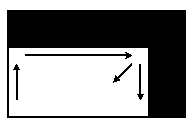
\includegraphics[scale=0.75]{Imagenes_Tutorial/10_Recursividad_1}
\end{center}

Empecemos por definir un rect\'angulo cuya altura y anchura dependan
de dos variables:
\begin{verbatim}
  para rectangulo :alto :ancho
    repite 2
      [ avanza :alto  giraderecha 90
        avanza :ancho giraderecha 90 ]
  fin \end{verbatim}
Para rellenar nuestro rect\'angulo, vamos a ejecutar:
\begin{verbatim}
  rectangulo 100 200 rectangulo 99 199 rectangulo 98 198 ... rectangulo 1 101  \end{verbatim}
\noindent algo que conseguimos de forma recursiva haciendo:
\begin{verbatim}
   para rectangulo :alto :ancho
      [ avanza :alto  giraderecha 90
        avanza :ancho giraderecha 90 ]
      rectangulo :alto-1 :ancho-1
   fin \end{verbatim}

Probando \texttt{rectangulo 100 200} nos encontramos con un problema:
el procedimiento no se detiene cuando el rect\'angulo se ha rellenado
por completo, sino que !`contin\'ua dibujando rect\'angulos! \\

Vamos a a\~nadir un condicional que permita detectar cuando la altura
o anchura son nulas. En ese momento, pediremos al programa que se
detenga con la primitiva \texttt{alto}:
\begin{verbatim}
 para rectangulo :alto :ancho
   si o :alto=0 :ancho=0 [alto]
   [ avanza :alto  giraderecha 90
     avanza :ancho giraderecha 90 ]
   rectangulo :alto-1 :ancho-1
 fin \end{verbatim}
Nota: En vez de utilizar la primitiva \texttt{o}, se puede utilizar el
s\'imbolo \char`\"{}\texttt{|}\char`\"{}, y escribir\'iamos:
\begin{verbatim}
  si :alto=0 | :ancho=0 [alto] \end{verbatim}

\section{Segundo intento}
   \label{sub:Segundo-intento}

% \input{Imagenes_pstricks/11_relleno2}
La idea aqu\'i va a ser que la tortuga empiece avanzando \texttt{100} pasos,
despues retroceda esos mismos 100 pasos; se desplace un poco a la
derecha y repita este movimiento, que llamaremos \char`\"{}elemental\char`\"{}
hasta que el rect\'angulo est\'e completamente coloreado.
\noindent \begin{center}
   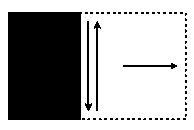
\includegraphics[scale=0.75]{Imagenes_Tutorial/11_Recursividad_2}
\end{center}

Si la altura del rect\'angulo est\'a representada por la variable \texttt{:alto},
ese ser\'a el movimiento elemental a repetir:
\begin{verbatim}
   avanza :alto retrocede :alto giraderecha 90 avanza 1 giraizquierda 90 \end{verbatim}
Este movimiento debe repetirse \texttt{:ancho} veces. El procedimiento
final ser\'a:
\begin{verbatim}
  para rectangulo :alto :ancho
    repite :ancho
      [ avanza :alto retrocede :alto
        giraderecha 90 avanza 1 giraizquierda 90 ]
 fin \end{verbatim}
Nota: si no se indica el primer trazo vertical en el bucle, har\'a un
peque\~no trazo de longitud un paso en la base del rect\'angulo.

Otro intento habr\'ia podido utilizar la recursividad y un condicional
como prueba de alcanzar el final.
\begin{verbatim}
   para rectangulo :alto :ancho
    si :ancho = 0 [alto]
    repite :ancho
      [ avanza :alto retrocede :alto
        giraderecha 90 avanza 1 giraizquierda 90 ]
   fin \end{verbatim}

Nota: A cada trazo vertical dibujado, disminuye la variable \texttt{:ancho}
en una unidad. As\'i pues, cuando vale \texttt{0}, se habr\'a dibujado el
rect\'angulo completo.

\section{Tercer intento}
   \label{sub:Tercer-intento}

% \input{Imagenes_pstricks/12_relleno3}
Efectuaremos los mismos movimientos que en la secci\'on anterior, pero
trazando consecutivamente l\'ineas horizontales:
\noindent \begin{center}
   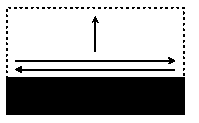
\includegraphics[scale=0.75]{Imagenes_Tutorial/12_Recursividad_3}
\end{center}
\begin{verbatim}
  para rectangulo :alto :ancho
    repite :alto
      [ avanza :ancho retrocede :ancho
        giraderecha 90 avanza 1 giraizquierda 9 ]
  fin \end{verbatim}

\newpage{}

\chapter{Actividad sobre las cifras de calculadora}
   \label{sec:Cifras-Calculadora}

% \input{Imagenes_pstricks/13_calculadora}
\begin{longtable}{m{10cm}m{6cm}}
Esta actividad se basa en el hecho de que todos los n\'umeros de calculadora
pueden obtenerse con ayuda de un patr\'on s\'i--no:
\begin{itemize}
   \item para dibujar un \char`\"{}4\char`\"{}, \char`\"{}encenderemos\char`\"{}
      los rect\'angulos 3, 4, 5 y 7, pero no los 1, 2 y 6
   \item para dibujar un \char`\"{}8\char`\"{}, \char`\"{}encenderemos\char`\"{}
      los rect\'angulos 1, 2, 3, 4, 5, 6 y 7.
   \item para dibujar un \char`\"{}3\char`\"{}, encenderemos los rect\'angulos
      2, 3, 4, 5 y 6, pero no los 1 y 7
\end{itemize} 
\section{El programa}
    \label{sub:Programa-Calculadora}

\noindent Nos basaremos en el rect\'angulo s\'olido de la secci\'on anterior: &
   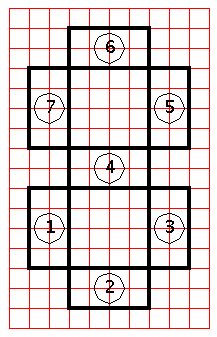
\includegraphics[scale=0.7]{Imagenes_Tutorial/13_Calculadora.png}
\end{longtable}

\begin{verbatim}
  para rectangulo :alto :ancho
    si :ancho = 0 | :alto =0 [alto]
    repite 2
      [ avanza :alto giraderecha 90
        avanza :ancho giraderecha 90]
    rectangulo :alto-1 :ancho-1
  fin \end{verbatim}
Supondremos aqu\'i que la tortuga parte de la esquina inferior izquierda.
Vamos a definir un procedimiento llamado \texttt{cifra} que lee 7
argumentos \texttt{:a}, \texttt{:b}, \texttt{:c}, \texttt{:d}, \texttt{:e},
\texttt{:f} y \texttt{:g}.
\begin{itemize}
   \item Cuando \texttt{:a} vale \texttt{1}, dibuja el rect\'angulo 1. Si
      \texttt{:a} vale \texttt{0}, no se dibuja.
   \item Cuando \texttt{:b} vale \texttt{1}, dibuja el rect\'angulo 2. Si
      \texttt{:b} vale \texttt{0}, no se dibuja.
   \item Cuando \texttt{:c} vale \texttt{1}, dibuja el rect\'angulo 1. Si
      \texttt{:c} vale \texttt{0}, no se dibuja.
   \item \ldots{}
\end{itemize}
Se obtiene el siguiente procedimiento:
\begin{verbatim}
 para cifra :a :b :c :d :e :f :g
 # Dibujamos el rectangulo 1
   si :a=1 [rectangulo 160 40]
 # Dibujamos el rectangulo 2
   si :b=1 [rectangulo 40 160]
   sl gd 90 av 120 gi 90 bl
 # Dibujamos el rectangulo 3
   si :c=1 [rectangulo 160 40]
   sl av 120 bl
 # Dibujamos el rectangulo 5
   si :e=1 [rectangulo 160 40]
 # Dibujamos el rectangulo 4
   gi 90 sl re 40 bl
   si :d=1 [rectangulo 160 40]
 # Dibujamos el rectangulo 6
   gd 90 sl av 120 gi 90 bl
   si :f=1 [rectangulo 160 40]
 # Dibujamos el rectangulo 7
   sl av 120 gi 90 re 40 bl
   si :g=1 [rectangulo 160 40]
 fin \end{verbatim}

\section{Creaci\'on de una peque\~na animaci\'on}

Vamos a simular una cuenta atr\'as, que consiste en hacer aparecer sucesivamente
las cifras de \texttt{9} a \texttt{0} en orden decreciente.
\begin{verbatim}
   para cuentatras
      bp ot cifra 0 1 1 1 1 1 1 espera 60
      bp ot cifra 1 1 1 1 1 1 1 espera 60
      bp ot cifra 0 0 1 0 1 1 0 espera 60
      bp ot cifra 1 1 1 1 0 1 1 espera 60
      bp ot cifra 0 1 1 1 0 1 1 espera 60
      bp ot cifra 0 0 1 1 1 0 1 espera 60
      bp ot cifra 0 1 1 1 1 1 0 espera 60
      bp ot cifra 1 1 0 1 1 1 0 espera 60
      bp ot cifra 0 0 1 0 1 0 0 espera 60
      bp ot cifra 1 1 1 0 1 1 1 espera 60
   fin \end{verbatim}
Peque\~no problema: hay un efecto de parpadeo desagradable durante la
creaci\'on de cada cifra. Para suavizarlo se van a utilizar las primitivas
\texttt{animacion} y \texttt{refrescar}. \texttt{animacion} hace que la
tortuga dibuje pero no lo muestre, es decir, a nuestros ojos no hace nada;
al recibir la orden \texttt{refrescar} muestra todo el trabajo almacenado en
memoria.

Para salir del modo \textit{animaci\'on} y volver al modo \textit{normal}
tenemos dos opciones:
\begin{itemize}
   \item Usar la primitiva \texttt{detieneanimacion} 
   \item Hacer \textit{click} en la c\'amara de cine que aparece a la
      izquierda del Hist\'orico de Comandos.
\end{itemize}

Se obtiene el siguiente programa modificado:
\begin{verbatim}
   para cuentatras
   # Entramos en modo animacion
     animacion
     bp ot cifra 0 1 1 1 1 1 1 refrescar espera 60
     bp ot cifra 1 1 1 1 1 1 1 refrescar espera 60
     bp ot cifra 0 0 1 0 1 1 0 refrescar espera 60
     bp ot cifra 1 1 1 1 0 1 1 refrescar espera 60
     bp ot cifra 0 1 1 1 0 1 1 refrescar espera 60
     bp ot cifra 0 0 1 1 1 0 1 refrescar espera 60
     bp ot cifra 0 1 1 1 1 1 0 refrescar espera 60
     bp ot cifra 1 1 0 1 1 1 0 refrescar espera 60
     bp ot cifra 0 0 1 0 1 0 0 refrescar espera 60
     bp ot cifra 1 1 1 0 1 1 1 refrescar espera 60
   # Volvemos al modo de dibujo habitual
     detieneanimacion
   fin  \end{verbatim}

\newpage{}

\chapter{Descubrir las listas y las variables}
   \label{sec:Listas-Variables}

\section{Interacci\'on con el usuario}
   \label{sub:Interaccion-Usuario}

Vamos a realizar un peque\~no programa que pide al usuario su nombre,
sus apellidos y su edad. Al final del cuestionario, el programa responde
con una lista del estilo:
\begin{verbatim}
   Tu nombre es: ........
   Tus apellidos son: ........
   Tu edad es: ........
   Tu eres mayor o menor \end{verbatim}
Para eso, vamos a utilizar las primitivas siguientes:
\begin{itemize}
   \item \texttt{leelista: \hspace{3.8cm}
      \textcolor{red}{leelista [?`Cu\'antos a\~nos tienes?] \char`\"{}a}}

      Presenta una caja de di\'alogo con el t\'itulo indicado en la lista
      (en este caso, titulada \texttt{?`Cu\'antos a\~nos tienes?}). El
      usuario da la respuesta y se guarda en forma de lista en la variable
      \texttt{:a}. Por ejemplo, si introducimos 20, la variable \texttt{:a}
      contendr\'a \texttt{[20]}.
   \item \texttt{haz: \hspace{5cm} \textcolor{red}{haz \char`\"{}a 30}}

      Asigna el valor 30 a la variable \texttt{:a}
   \item \texttt{frase, fr: \hspace{4cm} \textcolor{red}{frase [30 k] \char`\"{}a}}

      Incorpora un valor a una lista. Si este valor es una lista, acopla
      las dos listas.

      \begin{tabular}{lcl}
         \verb+frase [30 k] "a+ & ---> & \verb+[30 k a]+ \\
         \verb+frase [1 2 3] 4+ & ---> & \verb+[1 2 3 4]+ \\
         \verb+frase frase [1 2 3] [4 5 6]+ & ---> & \verb+[1 2 3 4 5 6]+ \\
      \end{tabular}
   \item \texttt{primero,\hspace{4cm}\textcolor{red}{pr}}:

      Devuelve el primer valor de una lista

      \begin{tabular}{lcl}
         \verb+escribe primero [4 5 6]+ & ---> & \verb+4+ \\
         \verb+escribe primero [Como te va 8]+ & ---> & \verb+Como+ \\
      \end{tabular}
\end{itemize}
\noindent Obtenemos el c\'odigo siguiente:

\noindent \texttt{para cuestion} \\
\texttt{leelista [?`Cuantos a\~nos tienes?] \char`\"{}edad} \\
\verb+    +\texttt{\# :edad contiene ahora una lista con un elemento;} \\
\verb+    +\texttt{\# extraemos ese elemento y lo guardamos de nuevo en :edad} \\
\texttt{haz \char`\"{}edad primero :edad} \\
\texttt{leelista [?`C\'omo te llamas?] \char`\"{}nombre} \\
\texttt{leelista [?`C\'omo te apellidas?] \char`\"{}apellidos} \\
\texttt{escribe frase [Te llamas: ] :nombre} \\
\texttt{escribe frase [Te apellidas: ] :apellidos} \\
\texttt{escribe frase [Tu edad es: ] :edad} \\
\texttt{si o :edad>18 :edad=18} \\
\texttt{[escribe [Eres mayor de edad]] [escribe [Eres menor de edad]]} \\
\noindent \texttt{fin}

\section{Programar un peque\~no juego}
   \label{sub:Pequeno-Juego}

El objetivo de este apartado consiste en crear el siguiente juego:
\begin{itemize}
   \item El programa elige un n\'umero al azar entre 0 y 32 y lo memoriza.
   \item Se abre una caja de di\'alogo y pide un n\'umero al usuario.
   \item Si el n\'umero introducido es igual al n\'umero memorizado,
      devuelve \char`\"{}\texttt{!`Acertaste!}\char`\"{} en la zona de
      texto.
   \item En el caso contrario, el programa indica si el n\'umero memorizado es
      \texttt{m\'as grande} o \texttt{m\'as peque\~no} que el n\'umero propuesto
      por el usuario
   \item Luego abre de nuevo la caja de di\'alogo.
   \item El programa se termina cuando el usuario ha encontrado el n\'umero
      memorizado.
\end{itemize}
\noindent Necesitar\'as utilizar la primitiva siguiente: \\

\texttt{azar}: \hspace{4cm} \textcolor{red}{\texttt{azar 20}}

Devuelve un n\'umero aleatorio entre 0 y 19. \\

\noindent VEAMOS ALGUNAS REGLAS QUE DEBES RESPETAR PARA REALIZAR ESTE JUEGO:
\begin{enumerate}
   \item El n\'umero se guardar\'a en la memoria del ordenador en una variable
      llamada \texttt{numero}.
   \item La caja de di\'alogo tendra por t\'itulo: \char`\"{}\texttt{Prop\'on un
      n\'umero:}\char`\"{}.
   \item El n\'umero introducido por el usuario ser\'a guardado en una variable
      llamada \texttt{prueba}.
   \item El procedimiento que inicia el juego se lanzar\'a con la palabra
      \texttt{juego}.
\end{enumerate}
ALGUNAS POSIBLES MEJORAS:
\begin{itemize}
   \item Limitar el n\'umero de intentos
   \item El n\'umero a adivinar debe estar comprendido entre 0 y 2000.
   \item Comprobar si el usuario introduce realmente un n\'umero o est\'a
      introduciendo una lista o una palabra. Para ello, utilizar la primitiva
      \texttt{numero?}

      Ejemplos:
      \begin{verbatim}
   numero? 8                  es cierto.
   numero? [5 6 7]            es falso. ([5 6 7] es una lista)
   numero? "abcde             es falso ("abcde es una palabra) \end{verbatim}
\end{itemize}

\newpage{}

\chapter{Una animaci\'on: \textit{El increible monigote creciente}}
   \label{sec:Monigote}

% \input{Imagenes_pstricks/14_monigote}
\noindent \begin{center}
   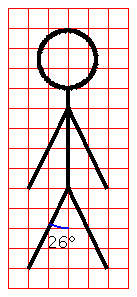
\includegraphics[scale=0.75]{Imagenes_Tutorial/14_Monigote.png}
\end{center}
En primer lugar, vamos a definir un procedimiento \texttt{monigote} que dibujar\'a
el monigote representado arriba, con un tama\~no de nuestra elecci\'on.
\begin{verbatim}
   para monigote :c
      gi 154 av 2.2*:c re :c*2.2
      gi 52 av 2.2*:c re :c*2.2
      gi 154 av :c*2
      gi 154 av 2.2*:c re :c*2.2
      gi 52 av 2.2*:c re :c*2.2
      gi 154 av :c/2
      gi 90 repite 180[av :c/40 gd 2] gd 90
   fin  \end{verbatim}

Vamos ahora con la animaci\'on que crear\'a la ilusi\'on de que el monigote
crece poco a poco. Para ello, escribimos \texttt{monigote 1}, despues
\texttt{monigote 2} \texttt{monigote 3} \ldots{} hasta \texttt{monigote
75}. Entre cada trazado, se borrar\'a la pantalla. Se obtienen los dos
procedimientos siguientes:
\begin{verbatim}
   para monigote :c
     si :c=75 [alto]
     gi 154 av 2.2*:c re :c*2.2
     gi 52 av 2.2*:c re :c*2.2
     gi 154 av :c*2
     gi 154 av 2.2*:c re :c*2.2
     gi 52 av 2.2*:c re :c*2.2
     gi 154 av :c/2
     gi 90 repite 180 [av :c/40 gd 2] gd 90
     bp ot monigote :c+1
   fin

   para empezar
      bp ot monigote 0
   fin \end{verbatim}

Por \'ultimo, para suavizar todo el proceso, vamos a servirnos del modo
\texttt{animacion} y de la primitiva \texttt{refrescar}.
\begin{verbatim}
   para monigote :c
     si :c=75 [alto]
     gi 154 av 2.2*:c re :c*2.2
     gi 52 av 2.2*:c re :c*2.2
     gi 154 av :c*2
     gi 154 av 2.2*:c re :c*2.2
     gi 52 av 2.2*:c re :c*2.2
     gi 154 av :c/2
     gi 90 repite 180 [av :c/40 gd 2] gd 90
     refrescar
     bp ot monigote :c+1
   fin

   para empezar
      bp ot animacion
      monigote 0
      detieneanimacion
   fin \end{verbatim}

\newpage{}

\chapter{Actividad sobre n\'umeros primos dos a dos}
   \label{sec:Actividad-Primos}

\noindent AVISO: Son necesarios algunos conceptos de matem\'aticas para comprender
bien esta secci\'on.

\section{Noci\'on de m.c.d. (m\'aximo com\'un divisor)}
  \label{sub:Nocion-de-m.c.d.}

Dados dos n\'umeros enteros, el m\'aximo com\'un divisor define al mayor
divisor com\'un de ambos. Por ejemplo:
\begin{itemize}
   \item 42 y 28 tienen como m.c.d. 14, ya que es el n\'umero m\'as grande por
      el que es posible dividir a la vez 28 y 42
   \item el m.c.d. de 25 y 55 es 5
   \item 42 y 23 tienen m.c.d. igual a 1
\end{itemize}
Cuando dos n\'umeros tienen m.c.d. 1, se dice que son primos entre s\'i.
As\'i en el ejemplo anterior, 42 y 23 son primos entre s\'i. Eso significa
que no tienen ning\'un divisor com\'un excepto 1 (!`por supuesto, hablamos
de divisi\'on entera!).

\section{Algoritmo de Euclides}
    \label{sub:Algoritmo-de-Euclides}

Para determinar del m.c.d. de dos n\'umeros, se puede utilizar un m\'etodo
llamado \textbf{algoritmo de Euclides}: (Aqu\'i no se demostrar\'a la
validez de este algoritmo, se admite que funciona)

He aqu\'i el principio: \char`\"{}dados dos enteros positivos \texttt{a} y
\texttt{b}, se comienza por probar si \texttt{b} es nulo. En caso afirmativo,
entonces el m.c.d. es igual a \texttt{a}. Si no, se calcula \texttt{r}, el
resto  de la divisi\'on de \texttt{a} por \texttt{b}. Se sustituye \texttt{a}
por \texttt{b}, y \texttt{b} por \texttt{r}, y se reinicia el m\'etodo.

Calculemos por ejemplo, el m.c.d. de 2160 y 888 por este algoritmo
con las siguientes etapas:
\begin{center}\ttfamily{\begin{tabular}{ccc}
   a   &  b  &  r \\
  2160 & 888 & 384 \\
   888 & 384 & 120 \\
   384 & 120 &  24 \\
   120 &  24 &   0 \\
    24 &   0 &
\end{tabular}} \end{center}
El m.c.d. de 2160 y 888 es, por tanto, 24. 24 es el mayor entero que
divide simult\'aneamente a los dos n\'umeros. De hecho, 
\texttt{2160 = 24 * 90} y \texttt{888 = 24 * 37}. El m.c.d. es, por tanto,
el \'ultimo resto no nulo.

\section{Calcular un m.c.d. en L{\small{OGO}}}
   \label{sub:m.c.d.-en-logo}

Un peque\~no algoritmo recursivo permite calcular el m.c.d. de dos n\'umeros,
\texttt{:a} y \texttt{:b}.
\begin{verbatim}
   para mcd :a :b
      si (resto :a :b) = 0
         [devuelve :b]
         [devuelve mcd :b resto :a :b]
   fin

   escribe mcd 2160 888\end{verbatim}
\noindent proporciona como resultado \texttt{24}

Nota: Nos vemos obligados a poner par\'entesis en \texttt{resto :a :b},
si no el int\'erprete intentar\'a evaluar \texttt{b = 0}. Para evitar este
problema de par\'entesis, podemos escribir: \texttt{si 0 = resto :a :b}

\section{Calcular una aproximaci\'on de $\pi$}
   \label{sub:Aproximacion-pi}

Un resultado conocido de teor\'ia de los n\'umeros pone de manifiesto
que la probabilidad que dos n\'umeros tomados aleatoriamente sean primos
entre ellos es de $\frac{6}{\pi^2} \simeq 0.6079$. Para intentar
encontrar este resultado, vamos a:
\begin{itemize}
   \item Tomar dos n\'umeros al azar entre 0 y 1 000 000.
   \item Calcular su m.c.d.
   \item Si su m.c.d. vale 1, anadir 1 a una variable contador.
   \item Repetir 1000 veces
   \item la frecuencia de los pares de n\'umeros primos entre ellos se obtendr\'a
      dividiendo la variable contador por 1000 (el n\'umero de pruebas)
\end{itemize}
\begin{verbatim}
  para prueba
  # Inicializamos la variable contador a 0
    haz "contador 0
    repite 1000
      [ si (mcd azar 1000000 azar 1000000) = 1
         [haz "contador :contador+1] ]
    escribe [Frecuencia:]
    escribe :contador/1000
  fin  \end{verbatim}

Nota: Igual que antes, nos vemos obligados a poner par\'entesis en

\texttt{mcd azar 1000000 azar 1000000}

si no, el interprete va a intentar evaluar \texttt{1 000 000 = 1}. Para evitar
este problema de par\'entesis, escribe:
\texttt{si 1 = mcd azar 1000000 azar 1000000}
\begin{verbatim}
   prueba
   0.609
   prueba
   0.626
   prueba
   0.597\end{verbatim}

Se obtienen valores pr\'oximos al valor te\'orico de 0,6097. Lo que
es notable es que esta frecuencia es un valor aproximado de 
$\displaystyle \frac{6}{\pi^2} \simeq 0,6079$.
Si tenemos en cuenta \texttt{f}, la frecuencia encontrada, se tiene pues:
$f\simeq\frac{6}{\pi^{2}}$. Despejando:
\[ \pi^2 \simeq \frac{6}{f} \quad \textrm{y as\'i:} \quad
   \pi \simeq \sqrt{\frac{6}{f}} \]

A\~nadimos esta aproximaci\'on al programa, y transformamos el final del
procedimiento \texttt{prueba}:
\begin{verbatim}
  para prueba
  # Inicializamos la variable contador a 0
    haz "contador 0
    repite 1000
      [ si (mcd azar 1000000 azar 1000000) = 1
         [ haz "contador :contador+1 ] ]
  # Tras calcular la frecuencia
    haz "f :contador/1000
  # Mostramos el valor aproximado de pi
    escribe frase [Aproximacion de pi:] raizcuadrada (6/:f) fin
  fin  \end{verbatim}
\noindent que proporciona:
\begin{verbatim}
prueba
Aproximacion de pi: 3.164916190172819
prueba
Aproximacion de pi: 3.1675613357997525
prueba
Aproximacion de pi: 3.1008683647302115 \end{verbatim}

Bien, modifiquemos el programa de modo que cuando lo lancemos, podamos
indicar el n\'umero de pruebas deseadas.
\begin{verbatim}
  para prueba :repeticiones
  # Inicializamos la variable contador a 0
    haz "contador 0
    repite :repeticiones
      [ si (mcd azar 1000000 azar 1000000) = 1
         [ haz "contador :contador+1 ] ]
  # Tras calcular la frecuencia
    haz "f :contador/:repeticiones
  # Mostramos el valor aproximado de pi
    escribe frase [Aproximacion de pi:] raizcuadrada (6/:f)
  fin \end{verbatim}
Probamos con 10000 repeticiones, y obtenemos en las tres primeras
tentativas:
\begin{verbatim}
prueba 10000
Aproximacion de pi: 3.1300987144363774
prueba 10000
Aproximacion de pi: 3.1517891481565017
prueba 10000
Aproximacion de pi: 3.1416626832299914 \end{verbatim}
\noindent No est\'a mal, ?`verdad?

\section{Compliquemos un poco m\'as: $\pi$ que genera $\pi$\ldots}
   \label{sub:Compliquemos-pi}

?`Qu\'e es un n\'umero aleatorio? ?`Es que un n\'umero tomado aleatoriamente
entre 1 y 1.000.000 es un n\'umero realmente aleatorio?

Deber\'ias darte cuenta r\'apidamente que nuestro modelo no hace m\'as que
aproximarse al modelo ideal. Bien, es precisamente sobre el modo de
generar el n\'umero aleatorio sobre el que vamos a efectuar algunos
cambios \ldots{}. No vamos utilizar m\'as la primitiva \texttt{azar},
sino que utilizaremos la secuencia de los decimales de $\pi$.

Me explico: los decimales de $\pi$ siempre han intrigado a los matem\'aticos
por su falta de regularidad, las cifras de 0 a 9 parecen aparecer
en cantidades aproximadamente iguales y de manera aleatoria. No se
pueden predecir los decimales siguientes bas\'andonos en los anteriores.

Vamos a ver a continuaci\'on como generar un n\'umero aleatorio con ayuda
de los decimales de $\pi$. En primer lugar, debes obtener los primeros
decimales de $\pi$ (por ejemplo un mill\'on). Existen dos programas
que los calculan bastante bien. Aconsejamos \texttt{PiFast} para Windows
y \texttt{ScnhellPi} para Linux.

Puedes acceder a Internet para conseguir un fichero de texto:
\begin{verbatim}
http://3.141592653589793238462643383279502884197169399375105820974944592.com \end{verbatim}
Tambi\'en en Internet, en la web de \textsc{XLogo}:
\begin{verbatim}
http://xlogo.tuxfamily.org/common/millionpi.txt \end{verbatim}

Para crear los n\'umeros aleatorios, agrupamos de 8 en 8 cifras la serie
de decimales de $\pi$. Es decir, el fichero empieza as\'i:
\[ \underbrace{3.1415926}_{\mathrm{1^{er}\ numero}}
   \underbrace{53589793}_{\mathrm{2^o\ numero}}
   \underbrace{23846264}_{\mathrm{3^{er}\ numero}}
   \underbrace{33832795}_{\ldots}0288419716939\ldots \]
Retiro la coma \char`\"{},\char`\"{} del \texttt{3.14\ldots} que podr\'ia
equivocarnos al extraer los decimales. Bien, todo est\'a preparado, creamos
un nuevo procedimiento llamado \texttt{azarpi} y modificamos ligeramente el
procedimiento \texttt{prueba}
\begin{verbatim}
 para mcd :a :b
   si (resto :a :b) = 0
    [ devuelve :b ]
    [ devuelve mcd :b resto :a :b ]
 fin

 para prueba :repeticiones
 # Abrimos el flujo numero 1 hacia el fichero millionpi.txt
 # (supongamos que se encuentra en el directorio de trabajo actual
 # si no estuviera, utilizar la ruta absoluta)
 # pondirectorio "/home/usuario/ruta_directorio
 # pondirectorio "c:\\Mis\ Documentos\ruta\ directorio
   abreflujo 1 "millionpi.txt
 # Asignemos a la variable "linea la primera linea del fichero millionpi.txt
   haz "linea primero leelineaflujo 1
 # Inicializamos la variable contador a 0
   haz "contador 0
   repite :repeticiones
     [ si 1 = mcd azarpi 7 azarpi 7
        [ haz "contador :contador+1 ] ]
 # Calculamos la frecuencia
   haz "f :contador/:repeticiones
 #  Mostramos el valor aproximado de pi
   escribe frase [Aproximacion de pi:] raizcuadrada (6/:f)
   cierraflujo 1
 fin

 para azarpi :n
   hazlocal "numero "
   repite :n [
 # Si no hay ningun caracter en la linea
   si 0=cuenta :linea
    [haz "linea primero leelineaflujo 1]
 # Asignamos a la variable :caracter el valor de primer caracter de la linea
   haz "caracter primero :linea
 # despues eliminamos el primer caracter de la linea
   haz "linea menosprimero :linea
   haz "numero palabra :numero :caracter ]
   devuelve :numero
fin \end{verbatim}
\noindent El resultado es:
\begin{verbatim}
prueba 10
Aproximacion de pi: 3.4641016151377544 
prueba 100
Aproximacion de pi: 3.1108550841912757 
prueba 1000
Aproximacion de pi: 3.081180112566604
prueba 10000
Aproximacion de pi: 3.1403714651066386 \end{verbatim}
% prueba 50000
% Aproximacion de pi: 3.137021734590537 

Encontramos pues una aproximaci\'on del n\'umero $\pi$ !`con ayuda de
sus propios decimales!\\

A\'un es posible mejorar este programa indicando por ejemplo el tiempo
usado para el c\'alculo. Se a\~nade, entonces, en la primera l\'inea del
procedimiento prueba:
\begin{verbatim}
 para prueba :repeticiones
   haz "principio tiempo
   ... \end{verbatim}
y se modifica el final del procedimiento
\begin{verbatim}
   ...
   cierraflujo 1
   escribe frase [ Tiempo empleado: ] frase tiempo - :principio "segundos
 fin \end{verbatim}

\newpage{}

\chapter{Actividad sobre la suma de dos dados}

Cuando se lanzan dos dados y se calcula la suma de los puntos de cada uno de
ellos, se obtiene un resultado comprendido entre 2 y 12. En esta actividad
vamos ver la distribuci\'on de frecuencias de las distintas tiradas y a
representarla en un sencillo gr\'afico.

\section{Simular el lanzamiento de un dado}

Para simular el lanzamiento de un dado, vamos a utilizar la primitiva
\texttt{azar}. Veamos c\'omo.
\begin{quote}
  \texttt{azar 6} ---> devuelve un n\'umero aleatorio comprendido
     entre 0 y 5.

  Por tanto, \texttt{(azar 6) + 1} devuelve una cantidad elegida aleatoriamente
  del conjunto \texttt{\{1,2,3,4,5,6\}}. \\

  Tener en cuenta la utilizaci\'on de los par\'entesis; si no, el int\'erprete
  \textsc{Logo} leer\'ia \texttt{azar 7}. Para evitar los par\'entesis, se puede
  escribir tambi\'en \texttt{1 + azar 6}.
\end{quote}
Se define as\'i el procedimiento \texttt{lanzar}, que simula el lanzamiento de un
dado.
\begin{verbatim}
 para lanzar
   devuelve 1 + azar 6
 fin \end{verbatim}

\section{El programa}

Vamos a utilizar el modo \textit{multitortuga}, para as\'i disponer de varias
tortugas sobre la pantalla.

Se utiliza la primitiva \texttt{pontortuga}, seguida del n\'umero de tortuga que
se quiere seleccionar.

Un buen esquema que vale m\'as que mil explicaciones \dots:
\begin{center}
   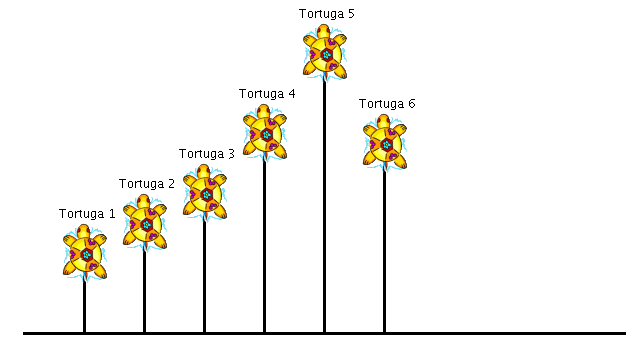
\includegraphics[scale=0.4]{Imagenes_Tutorial/15_Dados.png} 
\end{center}
El objetivo es que cada tortuga, numerada de 2 a 12, avance un
\textit{paso de tortuga} cuando el resultado de la suma de la tirada de los
dos dados coincida con su n\'umero. Por ejemplo, si la tirada de dados 
suma 8, la tortuga n\'umero 8 avanzar\'a un paso. \\

La separaci\'on horizontal entre las tortugas es de 30 pasos de tortuga, y se
colocar\'an a las tortugas con ayuda de los datos.
\begin{itemize}
   \item Se colocar\'a a la tortuga n\'umero 2 en \texttt{(-150 ; 0)}
   \item Se colocar\'a a la tortuga n\'umero 3 en \texttt{(-120 ; 0)}
   \item Se colocar\'a a la tortuga n\'umero 4 en \texttt{(-90 ; 0)}
   \item Se colocar\'a a la tortuga n\'umero 5 en \texttt{(-60 ; 0)}
   \item \dots
\end{itemize}
es decir:
\begin{verbatim}
 pontortuga 2 ponpos [-150 0]
 pontortuga 3 ponpos [-120 0]
 pontortuga 4 ponpos [-90 0]
 pontortuga 5 ponpos [-60 0]
 pontortuga 6 ponpos [-30 0]
 ...... \end{verbatim}
En lugar de copiar 11 veces pr\'acticamente la misma l\'inea de \'ordenes,
se puede automatizar utilizando la primitiva \texttt{repitepara}. Con ayuda
de esta primitiva, se puede asignar a una variable una serie de valores
distribuidos en un intervalo a espacios regulares. Aqu\'i, queremos que la
variable \texttt{:i} tome sucesivamente los valores \texttt{2, 3, 4, \dots, 12}. 
Su uso es:
\begin{verbatim}
  repitepara [i 2 12]
    [lista de las instrucciones que deben realizarse]
\end{verbatim}

\noindent Para colocar a las tortugas, se crea pues el procedimiento 
\texttt{inicia}
\begin{verbatim}
 para inicia
   borrapantalla
   ocultatortuga
   repitepara [i 2 12]
    [ # coloca la tortuga
     pontortuga :i ponpos lista -150 + (:i - 2) * 30 0
      # escribe el numero de la tortuga justo debajo
     subelapiz
     retrocede 15
     rotula :i
     avanza 15
     bajalapiz ]
fin \end{verbatim}

Observa la expresi\'on \texttt{-150 + (:i - 2) * 30}. Con ello hacemos que el
primer valor para la abscisa sea \texttt{-150}, y a cada nueva tortuga se
a\~naden 30 (probar con distintos valores de \texttt{:i} si no se ve bien). \\

\noindent Finalmente se obtiene el siguiente programa:
\begin{verbatim}
para lanzar
  devuelve 1 + azar 6
fin

para inicia
  borrapantalla
  ocultatortuga
  repitepara [i 2 12]
    [ # coloca la tortuga
     pontortuga :i ponpos lista -150 + (:i - 2)*30 0
      # escribe el numero de la tortuga justo debajo
     subelapiz
     retrocede 15
     rotula :i
     avanza 15
     bajalapiz ]
fin

para empezar
  inicia
# Hacemos 1000 intentos
  repite 1000
    [ haz "suma lanzar+lanzar
      pontortuga :suma 
      avanza 1 ]
 # indicamos las frecuencias de tirada
  repitepara [i 2 12]
    [ pontortuga :i
  # la ordenada de la tortuga representa el numero de tiradas
      hazlocal "frecuencia ultimo pos 
      subelapiz
      avanza 10 giraizquierda 90
      avanza 10 giraderecha 90
      bajalapiz
      rotula :frecuencia/1000*100 ]
fin \end{verbatim}

Veamos ahora una generalizaci\'on de este programa. Aqu\'i, se pedir\'an al
usuario el n\'umero de dados deseados as\'i como el n\'umero de lanzamientos
a efectuar.
\begin{verbatim}
para lanzar
  hazlocal "suma 0
  repite :dados
    [ hazlocal "suma :suma + 1 + azar 6 ]
  devuelve :suma
fin

para inicia
  borrapantalla ocultatortuga
  ponmaximastortugas :max + 1
  repitepara frase lista "i :min :max
   [ # coloca la tortuga
     pontortuga :i
     ponpos lista (:min - :max)/2*30 + (:i - :min)*30 0
     # escribe el numero de la tortuga justo debajo 
     subelapiz retrocede 15
     rotula :i
     avanza 15 bajalapiz ]
fin

para empezar
  leeteclado [Numero de dados:] "dados
  si no numero? :dados
   [ es [largoetiqueta El numero introducido no es valido!]
     alto ]
  haz "min :dados
  haz "max 6*:dados
  leeteclado [Numero de lanzamientos a realizar] "tiradas
  si no numero? :tiradas
   [ es [largoetiqueta El numero introducido no es valido!]
     alto ]
  inicia
# Hacemos un numero de intentos igual :tiradas
  repite :tiradas
    [ pontortuga lanzar
      avanza 1 ]
# indicamos las frecuencias de tirada
  repitepara frase lista "i :min :max
    [ pontortuga :i
  # la ordenada de la tortuga representa el numero de tiradas
      hazlocal "frecuencia ultimo pos 
  # normalizamos entre 0,1
      subelapiz
      avanza 10 giraizquierda 90
      avanza 10 giraderecha 90 bajalapiz
      rotula (redondea :frecuencia/:tiradas)*100 ]
fin \end{verbatim}

\newpage{}

\chapter{Soluci\'on a las actividades}

\section{Secci\'on \ref{sub:Actividad_Casa}}

\begin{verbatim}
para cuadrado
  repite 4 [av 150 gd 90]
fin

para tri
  repite 3 [av 150 gd 120]
fin

para puerta
  repite 2 [av 70 gd 90 av 50 gd 90]
fin

para chi
  av 55 gd 90 av 20 gd 90 av 20
fin

para desp1
  gd 90 av 50 gi 90
fin

para desp2
  gi 90 av 50 gd 90 av 150 gd 30
fin

para desp3
  sl gd 60 av 20 gi 90 av 35 bl
fin

para casa
  cuadrado desp1 puerta desp2 tri desp3 chi
fin \end{verbatim}

\section{Secci\'on \ref{sub:Actividad-Policubos}}

\begin{verbatim}
para supercubo
  bp sl ponpos [-30 150] bl
  ponpos [-150 150]  ponpos [-90 210]  ponpos [30 210]  ponpos [-30 150]
  ponpos [-30 -210]  ponpos [30 -150]  ponpos [30 -90]  ponpos [-30 -90]
  ponpos [90 -90]    ponpos [90 30]    ponpos [-270 30] ponpos [-270 -90]
  ponpos [-210 -90]  ponpos [-210 -30] ponpos [-90 -30] ponpos [-90 -150]
  ponpos [-210 -150] ponpos [-210 -30] ponpos [-150 30] ponpos [-30 30]
  ponpos [-90 -30]   ponpos [90 150]   ponpos[30 150]   ponpos[30 210]
  ponpos [30 90]     ponpos [90 90]    ponpos [90 150]  ponpos[90 90]
  ponpos [150 90]    ponpos [150 -30]  ponpos[90 -90]   ponpos[90 30]
  ponpos [150 90]
  sl ponpos [-150 30] bl
  ponpos [-150 150]  ponpos [-150 90]  ponpos [-210 90] ponpos [-270 30]
  sl ponpos [-90 -150] bl
  ponpos [-30 -90]
  sl ponpos [-150 -150] bl
  ponpos [-150 -210] ponpos [-30 -210]
fin \end{verbatim}

\section{Secci\'on \ref{sub:Actividad-Robot-Rana}}

\subsection{El robot}
   \label{sub_El-Robot}

El primer dibujo est\'a formado exclusivamente por un motivo elemental
basado en un rect\'angulo, cuadrado y tri\'angulo. He aqu\'i el c\'odigo asociado
a este dibujo:
\begin{verbatim}
para rec :alto :ancho
# dibuja un rectangulo de altura :alto y anchura :ancho
  repite 2 [av :alto gd 90 av :ancho gd 90]
fin

para cuadrado :c
# dibuja una cuadrado de lado :c
  repite 4 [av :c gd 90]
fin

para tri :c
# dibuja un triangulo equilatero de lado :c
  repite 3 [av :c gd 120]
fin

para piernas :c
  rec 2*:c 3*:c cuadrado 2*:c
fin

para antenas :c
  av 3*:c gi 90 av :c gd 90 cuadrado 2*:c
  sl re 3 *:c gd 90 av :c gi 90 bl
fin

para robot :c
  bp ot
# El cuerpo
  rec 4*:c 28*:c
# Las piernas
  gd 90 av 2*:c
  piernas :c av 4*:c
  piernas :c av 14*:c
  piernas :c av 4*:c
  piernas :c
# La cola
  sl gi 90 av 4* :c bl
  gd 45 av 11*:c re 11*:c gi 135
# el cuello y la cabeza
  av 18*:c cuadrado :c
  av 3*:c cuadrado :c
  gd 90 av :c gi 90 av 3*:c gd 90
  cuadrado 8*:c
# Orejas
  av 4*:c gi 60 tri 3*:c
  sl gd 150 av 8 *:c gi 90 bl tri 3*:c
# Las antenas
  av 4 *:c gi 90 av 2*:c gd 90 antenas :c
  gi 90 av 4*:c gd 90 antenas :c
# los ojos
  sl re 3 *:c bl cuadrado :c
  gd 90 sl av 3*:c bl gi 90 cuadrado :c
# La boca
  sl re 3*:c gi 90 av 3*:c gd 90 bl rec :c 4*:c
fin \end{verbatim}

\subsection{La ranita}

\begin{verbatim}
para rana :c
   bp ot
   av 2 *:c gd 90 av 5*:c gi 90
   av 4*:c gi 90 av 7 *:c gd 90
   av 7*:c gd 90 av 21 *:c gd 90
   av 2*:c gi 90 av 2*:c gd 90
   av 9*:c gd 90 av 2*:c gi 90
   av 2*:c gd 90 av 9*:c gd 90
   av 2*:c gd 90 av 7*:c re 5*:c gi 90
   av 4*:c gd 90 av 4*:c re 4*:c gi 90
   re 2*:c gi 90 av 5*:c gi 90 av 4*:c gd 90
   av 7*:c gd 90 sl av 9*:c bl
   repite 4 [av 2*:c gd 90]
fin \end{verbatim}

\section{Secci\'on \ref{sub:Pequeno-Juego}}

\begin{verbatim}
para juego
# Inicializamos el numero, contador y el programa
  haz "numero azar 32
  haz "contador 0
  bucle
fin

para bucle
  leelista [Propon un numero: ] "prueba
  si numero? :prueba
# Si el valor introducido es un numero
   [ si :numero = :prueba
      [es fr fr [Has ganado en ] :contador+1 [intento(s)!] ]
      [ si :prueba > :numero
         [es [Mas pequeno] ]
         [es [Mas grande] ]
      haz "contador :contador+1
      bucle ]  ]
  [ escribe [Debes introducir un numero valido!]
    bucle ]
fin \end{verbatim}

\end{document}
